\section{Optimization Pitfalls}
\emph{Efficient} optimization of reduced neuron models is shockingly non-trivial, although satisficing biologically plausible models is several degrees easier.
Below I provide a number of examples of optimization pitfalls which were not obvious at the start of my research, but which I discovered during my research, and which were on ongoing source of confusion, not just for me, but for my whole research team.
I believe that it is important to share these conceptual traps with my readership, including those who may wish to continue such optimization work.

Genetic algorithms are favorable because they provide a good solution to the exploration/exploitation trade-off. If not hunting for a new prime number few are able or willing to wait out their whole lifespan to obtain the scientific results that there career depends on. There are steeply limited budgets for exploring solution spaces, therefore it seems prudent to accept solutions which are are not optimal but are negligently close to optimal. Often however, we may be interested in problems with complex and unlearn-able error surfaces that effectively "bury" the optima in noise. In such a cases it may be acceptable to obtain merely a satisfactory solution, in this context, the highest objective is to recover "biologically plausible models" and many fitted models can easily surpass this lower criteria of acceptable optimization.

Fortunately the coupling of neuronunit to a Genetic Algorithm facilitates either optimizing or a silent falling back to satisficing as appropriate. The term "satisfice" means that a measured property is either deemed satisfactory or optimal \cite{simon1956rational}. Although we may not know if a true optima is missed, neuronunit is often able to report if a solution is satisfactory. Forinstance when using neuroelectro data we can check if a model is biologically plausible, by consulting the models $\chi^{2}$ statistic over a collection of different electrical measurements.  Assuming that underlying experimental data is normally distributed as discussed in \ref{section:data-sources}. In addition to near optimal and satisfactory model fits models may also fail to achieve even a satisfactory fit and in that case it is helpful to quantify the degree of fitness failure.

% (occasionally the data my violate the assumption of normally distributed)
%The term satisficing, a portmanteau of satisfy and suffice,[2] was introduced by Herbert A. Simon in 1956,[3]
% XXXX Fill in all figure captions

\subsection{Is Optimization Always Possible?} 
For optimization to both succeed and be useful, several criteria must be met \cite{van2007neurofitter}:
\begin{itemize}
\item Relevance: The objective function should reflect fundamental and important properties of the data that a good model would reproduce.
\item Speed: The objective function should be fast to calculate, since typically a large number (potentially millions) of evaluations are performed during the search, many of which may require re-simulation of the model.
\item Efficient Convergence: The solution space should be as continuous and convex as possible, so that the search algorithm can rapidly converge to a global optimum.
\end{itemize}

%The EFEL signal processing suite was able to produce measurements that fulfilled the speed criteria. 

\subsubsection{Relevance of the objective function}
Due to the abundance and diversity of data available through the NeuroElectro Project \cite{tripathy2014neuroelectro}, my initial work relied heavily on that data source.
However, that data is enriched in passive membrane properties as well as the details of individual action potential waveforms.
But what distinguishes, say, a Layer 5 pyramidal cell in motor cortex from a Layer 5 pyramidal cell in visual cortex, in terms of the computational principles that systems neuroscientists might care about (e.g. decoding, information, etc.) is more likely to be reflected in the patterns of spiking and not the dynamics of single spikes or subthreshold behavior.
Furthermore, most reduced models are not implemented in way that allows for richly detailed action potential waveforms to be reproduced.
Together, this implies that reduced models optimized against data exclusively from NeuroElecto may be the worst of both worlds: they fail to capture the sub-millisecond dynamics of the action potential encoded in that data, while also failing to exhibit any of the suprathreshold dynamics (e.g. types of bursting) that distinguish one cell type from another, in the mind of a systems neuroscientist.
This problem is mitigated by including complementary data sources (like the Allen Cell Types database) that can address these dynamics.
Future optimization efforts should take care to identify the data sources that capture the dimensions of the experimental data along which meaningful differences between cell types can be resolved, and which models are rich enough to express.


\subsubsection{Speed of the objective function}
A large fraction of the compute cycles spent evaluating each parameter set are expended on identifying the rheobase current, thus unlocking the calculation of several subsequent measurements.
Fortunately, for slower model implementations this can be sped up significantly through parallelism, as described in section \ref{sec:parallel-rheobase}. BluePyOpt uses a python library pebble to in order to evaluate chromosomes in parallel. Often parallel code scheduling interfered with numba jit code, and so code logic must be applied to designate model specific speed up strategies. 

\subsubsection{Computational and Algorithmic Factors That Impinge on Convergence}

%In addition to words like ``stack" and ``heap", computer scientists distinguish between two types of memory: Its common for computer scientists RAM usually just termed ``memory", and disk. 

In this work it was sometimes memory pressure and not time pressure that prohibited the acquisition of results. This was especially true when mining features from pre-existing databases. In contexts where memory exhaustion routinely lead to program failure another code technique were applied to remedy the situation. A tool: Dask \cite{rocklin2015dask} facilitates the creation of big data set focused recipes. In this context a dask "delayed" iterator, provides a means to "stream" very large collections of data while only storing smaller chunks of the data in memory (RAM) as they are needed elsewhere in a program. This kind of data juggling might sound like common sense, but usually when data sizes are normal storing data out of memory (on disk) leads to significant slowdowns, and achieving a timely juggling of data between disk and memory is non trivial. % The code idiom that facilitates delayed evaluation is a method with a "$@$delayed" function decorator. 
%Delayed evaluation is intrinsically multi-threaded (but not multiprocessor), so delayed functions experience only intermediate speed-ups. 
Additionally delayed evaluation caused fewer conflicts with \emph{jit} code. With all of these issues in mind, implementing parts of the PhD project necessitated model dependent switching between the tools as follows: 
\begin{verbatim}numba-only, numba+delayed, pebble-only, delayed-only\end{verbatim} etc. This may seem overly complex but other formulations would not have resulted in timely memory friendly computations.


%timlyness of results was not the fundamental 
%Additionally the dask delayed algorithm
%In this context there were two different classes of model: 
%Models that should have parallel Rheobase or parallel chromosome evaluation.

%Caching of simulation results can also speed up evaluation, for example when computing multiple features based upon the same simulated membrane potential trace (e.g. spike count and time to first spike at a given current amplitude).
% Although this is an obvious opportunity for speed up, it was abandoned as the first pass attempt at solving this inside Neuronunit lead to unpredictable bugs for the whole team of programmers involved. This would probably work in current versions of neuronunit.
%XXXX More about speed here.

\subsubsection{Factors That Facilitate Efficient Convergence}
Place holder


\subsubsection{Continuity of the Error Surface}
Some optimization techniques require a perfectly convex error surface to converge.
Genetic algorithms are more tolerant, up to a point, but an extremely high dimensional optimization problem with a large number of optima can still be intractable.
Even more problematic are discontinuous error surfaces, which result naturally from bifurcations in the underlying dynamical system.
In this work, I grappled with two types of error surface defect. Some error surfaces that were highly "corrugated", a term I have coined to describe surfaces low amplitude oscillatory disturbances across the error surface. In addition to corrugation occasionally discontinuties in the surface were present, the causes of these abrupt jumps in surface value were easier to understand however.  

As stated above the amplitude of the error surface disturbances was relatively small, this meant it was possible for humans to conceptualize the surface defects as low amplitude noise.
Unfortunately this did not mean it no longer a problem for the genetic algorithms. NSGA2 a type of genetic selection ranks solutions according to a principle of non-domination, where improvements to fitness must co-occur. Under this scheme the best chromosomes are the ones where all fitness criteria improve together. Potentially fitter solutions are penalized, if some improvements occur at the expense of other criteria. Unfortunately the principles of this algorithm imply that it is not sensitive to the amplitude of error improvements, as it only senses the sign of relative improvement: "positive" or "negative". Therefore NSGA2 has a greater propensity to become fixated with the basins of the low amplitude corrugations. Unlike NSGA2 IBEA was better able to distinguish big from small and it was more resilient to getting stuck in these low amplitude surface defects. 

It is possible that permitting dominating errors to occur is helpful for guiding chromosomes uphill against error when leaving a local minima. When experiencing dominant error improvements, initially only one fitness value goes down dramatically at the expense of others which may get worse. If the lip of a valley is exists in all but one dimension, domination combined with mutation, may make for a push-pull type effect, that better facilitates uphill exploration. 

Another way to think about this is, the simple select-best algorithm may better facilitate moving up over a lip of a valley to then fall into gravity other error wells, were soon after all errors are able to fall together.

% DISCONTINUITIES -> IRREGULARITIES.  not sure that these are discontinuties. To use tectonic metaphors: A discontinuity is like misaligned tectonic plate after an earth quake. A corrogation can be smooth like a sinewave, or pond ripple.


If most components of the multi-objective functions, i.e. the outputs from tests of single features, were continuous then the inclusion of a very small number of corrugated error functions did not prohibit successful optimization.
However, inclusion of too many corrugated function proved problematic.

\subsection{Error Surfaces}
In methods I describe two approaches to fitting models, one of those approaches involved a supra-threshold virtual experiment that guides optimization, in models when more than one spike is measured. The other approach involves an at-threshold virtual experiment that guide optimization, where one or no spikes are expected.

It is important to know which approach resulted in the smoothest and most tractible error surfaces. Below I plot error surfaces from each kind of paradigm, such that the reader can also asses which surface look more useful for optimisation. 

Case 1, Izhikevich model at threshold virtual experiment. Constraints used:
\begin{verbatim}
TimeConstantTest,RestingPotentialTest,InputResistanceTest, CapacitanceTest, FITest
\end{verbatim}

All the figures below employ a consistent color coding scheme where red encodes the highest error and blue the lowest error. Because the reduced neuronal models are high dimensional the easiest way to view the error surface the models experience under optimization is to make 2D plots of their surface for each different pairings of $12$ model parameters.

%The surface plot from the supra threshold paradigm shows more contrast for two reasons: 1, it has less intermediary values (light green colour), reason two, it less high frequency changes, or ripples in the error surface.  


\begin{figure}
    \centering
    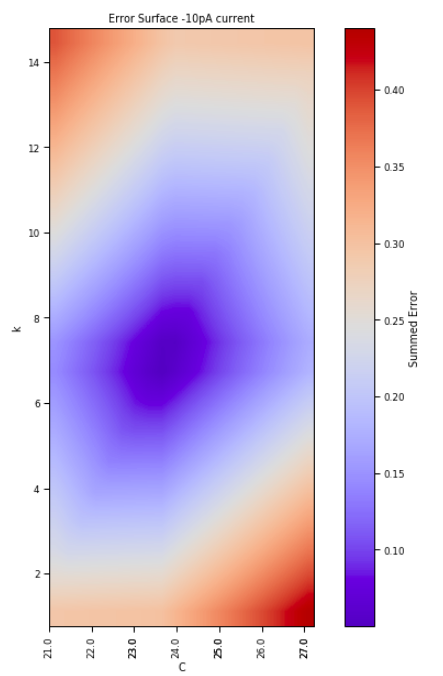
\includegraphics[scale=0.7]{figures/friendly_error_surface.png}
    \caption[Using only constant currents causes simple tractable error surfaces]{Because a constant current injection of $-10pA$ was applied, the error surface is simple informative and very easy to navigate, although only one slice into the error hypervolume is shown. Plots of GA learning speed provide also demonstrate that the error surface is free from both corrogations and discontinuties. Other plots (not shown here) demonstrate that all other slices into the hypervolume have simple convex shape.}
    \label{fig:constant_current}
\end{figure}


Case 2, AdExp Model model supra-threshold virtual experiment. Constraints used:
\begin{verbatim}
adaptation_index,adaptation_index2 time_to_first_spike, mean_AP_amplitude,spike_half_width, AHP_depth,minimum_voltage,peak_voltage,time-to-last-spike,AHP-depth-abs,all_ISI_valuesvoltage_base, min_voltage_between_spikes,Spikecount
 \end{verbatim}
\begin{figure}
    \centering
    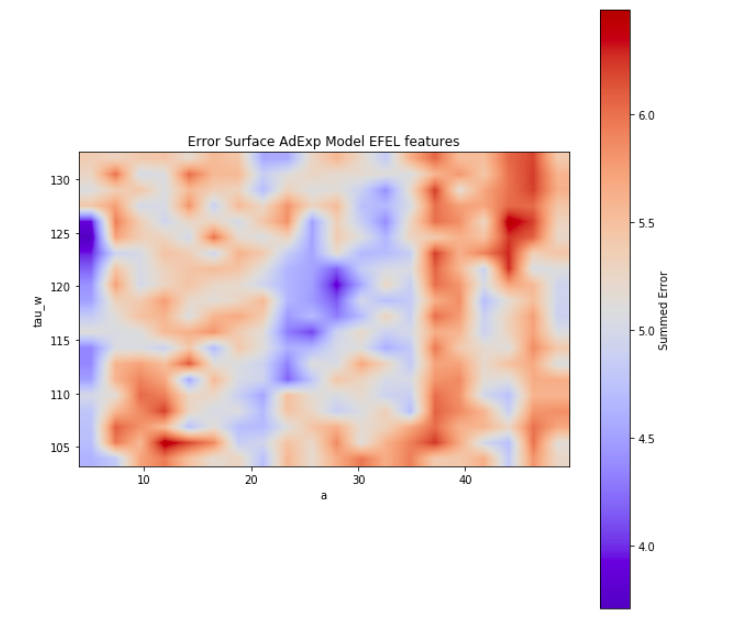
\includegraphics[scale=1.25]{figures/adexp_efel_problem.png}
    \caption[A very complicated but not hopeless error surfaces]{A two dimensional error surface drawn from summed EFEL error scores, acting on Adaptive Exponential models.
    
    The optima chosen by the optimizer was actually the one in the centre, and not the one on the left, bear in mind, however, that these are only two out of approximately 12 model dimensions, and these two dimensions may not have weighed heavily in the final summed score (as opposed to the component error depicted here)}
    \label{fig:real_problem_nontrivial_surface}
\end{figure}

\begin{figure}
    \centering
    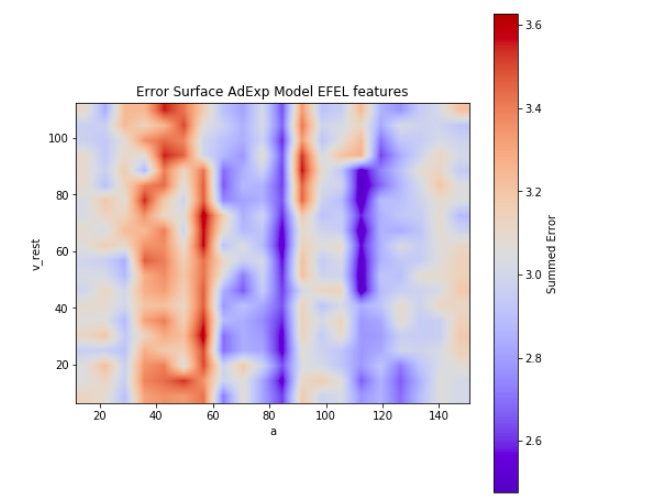
\includegraphics[scale=1.25]{figures/third_error_surface.png}
    %\caption[Cliff ledge in 2D error surface]{Cliff ledge in 2D error surface}
        \caption[Complex but not hopeless error surfaces]{Complex error surface with alternating neighbouring ridges and valleys (ripples)}
    \label{fig:real_problem_nontrivial_surface}
\end{figure}



% dont need to share complexity with reader.
%Although not shown here a third case is worth describing, as this third test combination achieved many useful results: Izhikevich model at threshold virtual experiment. Constraints used:
%\begin{verbatim}
%Case1 + RheobaseTest,
%\end{verbatim}


\subsubsection{Number of Components in the Objective Function}
Theoretically every additional component included in the objective function--every constraint derived from some experimental feature--should make the error surface a better answer to the question, "Is this a realistic model of the neuron of interest?".
While increasing computation time per objective function evaluation, such components may rapidly exclude large volumes of parameter space from unnecessary exploration.
For example, when modeling a bursting neuron, including burst-statistics as one of the features under evaluation will quickly exclude non-bursty regions of parameter space from consideration.
And yet a successful optimization recipe should not naively involve the use of all available computable features.


Some features might be biologically irrelevant, or impossible for some model class to reproduce, or have extremely discontinuous error surfaces.
%%%
%
This makes the task of optimization less automatic--careful human guidance is needed to curate the appropriate features for the task. 
%%%
%OR DOES IT?
I suspect that other pre-existing optimizers that fit neuronal models are often satisficing and not so much learning the error surface. Without having available graphs of other GA learning speeds we cannot know if existing models find their best fits via genuine learning, or via random search. In other words we can't tell when an optimizer finds an optimal or satisfactory model via random sampling, and besides such "satisficing" is legitimate GA behavior.
%%%

Genetic Algorithms are preferred over exhaustive search, because they use learning to sparsely and efficiently sample an otherwise prohibitively large space. Unfortunately, efficient optimization often warrants a small cursory grid search of the parameter space, and this grid search introduces circularity back into methodology. What we wanted was a way to avoid the exhaustive search, and therefore the optimizer must be able to search autominously.
% NB, this is harder to understand than the residual rheobase error idea.    
\subsubsection{Contingent Discontinuities}




Some tests used to compute the objective function may depend on the results of other tests.
They may depend on the measured value of one feature, for example, a test of the action potential width at half-height depends on the height measured from threshold which depends on the threshold.
Or they may depend on a stimulus parameter derived from a previous test; for example, computing the first inter-spike interval (ISI) at 1.5x rheobase first requires computing rheobase, and then multiplying the rheobase value by 1.5 to generate the stimulus for the ISI test.
Such an ISI test--and its results--is thus "contingent" on the results of the rheobase test.
This has confounding implications.
Suppose that as some model parameter $X$ is increased, the cell becomes more excitable.
All things being equal, more excitability would be associated with a lower rheobase, and with a narrower first inter-spike interval at a fixed current.
But because the rheobase determines the value of the actual current injected in the ISI test (the ISI test is contingent), the ISI could go up or down; it would go down if the direct effect of greater excitability associated with increased $X$ dominates; it would go up if the indirect effect of a smaller current injection dominates.
In fact, it is impossible (or at least impractical) to predict which of these will "win", and the resulting error surface for the ISI test becomes extremely corrugated.
The problem is even more extreme when the contingent test can produce missing values.
An ISI test depends on their being an inter-spike interval to measure, i.e. it requires a second spike to be produced.
If there is no second spike, this test will emit a missing value.
Thus as $X$ is increased, the error surface associated with the ISI test will be pocked with missing values every time the underlying change in excitability is offset too much by the ensuing change in rheobase-derived injected current.
And an error surface plagued with too many missing values is essentially unusable.
These contingent discontinuities present a major problem to the logic of contingent testing that underlies most of the optimization presented here.

\begin{center}
\begin{figure}
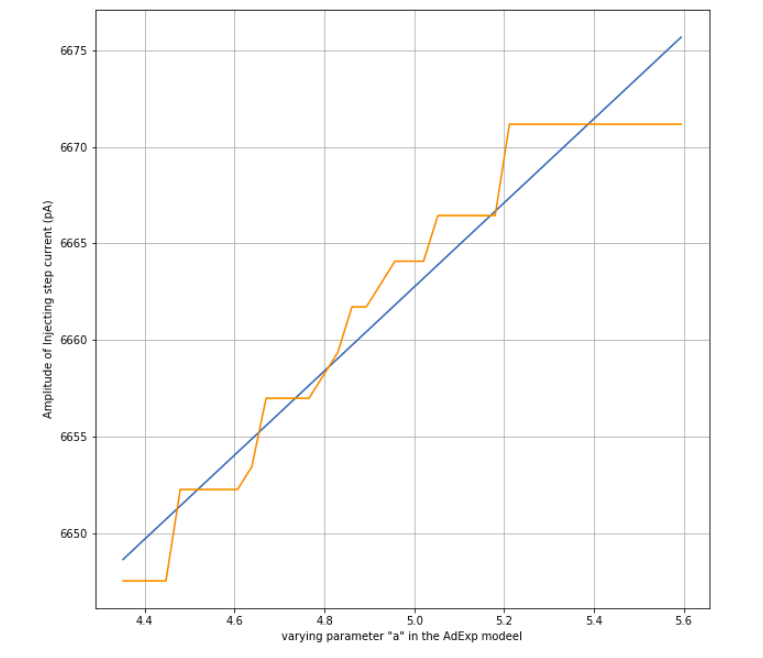
\includegraphics[]{figures/fundamental_cause_of_corrogations.png}
\caption[]{The main cause of corrugated error surfaces in this work was found to be re-calculating required currents on a model by model basis. In this plot the model was forced to fire exactly 11 spikes while the value of 'a' was swept between $4.4$-$5.6$, a straight line given by linear regression, approximates where we expect required current injection amplitude to fall, but instead, the real value routinely deviates on either side of the straight line. Upper and lower deviations represent a small but measurable current "excesses" that are free to propagate into other measured features of spiking waveforms where they amplify. By necessity the rheobase determining algorithm utilized in this work has a finite precision. So although in theory rheobase is defined as the minimum current amplitude to cause exactly one spike, in practice there will be small variable amounts of excess current injection strength. Such propagating errors were applied to many threshold dependant waveform features. Its important to note that because resulting corrugations were smaller in amplitude than other important features of the error surface. Humans can conceptualize the small amplitude corrugations as noise. Optimization in the presence of such noise sources was often viable, but in such a case, successful optimization becomes contingent on the satisfaction of other favorable conditions}
\label{fig:contingent_discontinous}
\end{figure}
\end{center}


One solution is make tests depend on a static value of rheobase sourced directly from the experimental data, rather than using the rheobase which belongs uniquely to the current models parameter set.
In other words, if the rheobase of the biological neuron is 100 pA, then the $1.5\times$ rheobase ISI test should be performed with a current injection of 150 pA, even if the rheobase of the current model parameterization is some entirely different value.
In practice this is less costly than optimizing over an intractable, corrugated error surface.

%%
% No! I think this would exclude space quicker and therefore save time. it would not cost time.
%%%
%In principle, this means wasting a bit of extra computation time exploring some poorly-fitting parameter sets, but 

Another approach is to dispense with the rheobase entirely, and simply test using a fixed set of current amplitudes that span the suprathreshold portion of the F-I curve, e.g. 200pA, 350pA, and 500 pA for a typical neuron.
This seems extremely direct, but it in some cases it fails to explore the most interesting peri-threshold portion of the F-I curve, where the dynamics of single spikes contain a great deal of information about peri-threshold dynamics.
For example, an after-hyperpolarization that is visible after single spike at rheobase may become completely swamped by the combination of inward pipette current and sodium current at values of injected current that are high above threshold.

\subsubsection{Inconsistent feature calculation algorithms}
The NeuronUnit core, the Ephysiology Feature Extraction Library \cite{EFEL}) EFEL, the Allen SDK, and the tests derived from \cite{druckmann2008evaluating} all contain independently written algorithms for computing features from simulated membrane potentials.
In some cases, the same feature (e.g. action potential threshold) is computed in many different ways across these feature extraction libraries.
All compute the threshold by first taking the first difference of the membrane potential, but they differ in subsequent steps, for example what value the first difference must reach to be considered at or beyond threshold.
This is inconvenient, but one can simply select one (or more) of the alternatives and apply it consistently.
More troubling are the cases where these algorithms differ in the stimulus used to generate the feature.
For example, the suprathreshold tests of \cite{druckmann2008evaluating} are based on a multiple of rheobase (e.g. $1.5\times$ or $3\times$), whereas those used by The Allen Insitute are based on additive increments from rheobase (e.g. +20 pA or +40 pA).
This means that cannot simply be applied to the same membrane potential trace, as those who collected the experimental data are likely to have chosen either multiples or additive increments of rheobase, but not both, depending on which lab they happen to work for.

As discussed in \ref{sec:methods}, I use code to restructure Allen and BlueBrainProject sweep data sets, where I sort traces into approximate multiples of rheobase. To make these conflicting lab protocols interoperable I impute 1.5 $\times$ and 3 $\times$ rheobase where it was not provided by finding the stimulus sweep pair that is the closest approximation. In this way I find the nearest traces to those predicted values in the Allen and BBP collections of sweeps. However, one can conceive of more mathematically savvy types of imputation, that achieve much greater levels of accuracy by weighting components of the two closest waveforms together, according to eachs distance from the required current injection value. In this way I assumed it was possible to generate predicted features from one stimulus convention based on observed features from the other, meaning that via imputation I had obtained an full (but approximated) set of features across the differing lab protocols.

%that is what I mean when I write imposing a new organisation on the sweep data.

% It may be possible to generate predicted features from one stimulus convention based on observed features from the other, allowing imputation of a full set of features across all algorithms, but this is beyond the scope of my thesis work. ISNT THIS WHAT I DID IN SOMEWAYS? IF I COULDN"T COMPARE ACROSS LAB PROTOCALS THEN THE ANALYSIS I DID WAS POINTLESS WAS IT NOT?

\subsection{Objective Function Dimensionality vs Model Parameter Dimensionality}    
Another pitfall arises when the the number of independent, reliable tests used to generate the objective function is small (or at least not large) relative to the number of parameters in the model being optimized.
Genetic algorithms are known as derivative-free optimizers, since they do not follow any gradient down the error surface, or even know of the existence of such a gradient.
Chromosomes only survive and reproduce differentially according to their location on the error surface.
Genetic optimization is never truly "stuck" inside a local minima on the error surface, as mutation or crossover can always produce new chromosomes outside the basin of attraction. Despite this robustness, just like in gradient descent, genetic algorithms can only be guided by information in the error surface.
When the objective function has a low-dimensionality, for example when it is based upon tests that mostly compute small variations on the same small number of features of the simulation output, it may not provide enough information to distinguish one location in parameter space from another one close by, even though the first may be closer to the optimal solution than the second.
In other words, many regions of parameter space may be locally flat at a mesoscopic scale, and local minima at a microscopic scale may thus be difficult to escape.
No lower error solution may be available within a reasonable distance (in parameter space) from the current one.

\subsection{More about Rastrigin's function...?}
Rastrigin's function has convexity in two scales. On the larger scale the surface has a convex property, on the small scale the function is uniformly pocked with minima wells. In order for the GA to optimize Rastrigin's function it must be able to exploit the global information of the error surface, and simultaneously the genes will often converge for generations in the minima, but they won't get stuck there for two reasons: Reason 1, the global convex shape will be represented in some genes that participate in cross over, therefore it is learnable. Reason 2:
 mutation and cross-over provide a significant repulsive force, driving chromosomes to test other locations despite that they perceive those locations to be less optimal.\\
   %\begin{figure}
  %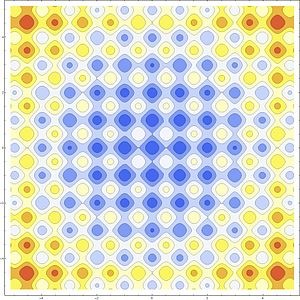
\includegraphics[]{figures/rastagrind.jpg}
  %\caption{}
   %\end{figure}
   
   It is worth noting that although Rastrigrins function is challenging it does not the present the worst gradient to learn from. Worse than Rastrigrins function, are functions that on a large scale are flat, but on the smaller scale contain a high density ripples.
   but lacks this global convex trend, excepting for an abrupt and localised descent to the optima.
   
   Without some first prior knowledge of the error surface, a likely outcome is to attempt optimize on uninformative surfaces. If an uninformative surface is applied, it does not mean that the genetic algorithm will not succeed, it only means that the performance of the GA may be only marginally better than random sampling, or exhaustive search of the error surface.
   %Random sampling, sounds bad, however, if the best random solution is digitally stored, and the number of samples applied is less than the possible number of samples in an exhaustive search, random sampling may better resolve the exploitation/exploration dilemna than both gradient descent, and exhaustive search.

\subsection{Specific examples of challenging real-world error surfaces encountered in this work}
In the figures below, I describe the spectrum of error surface quality.
\begin{figure}
\begin{center}
     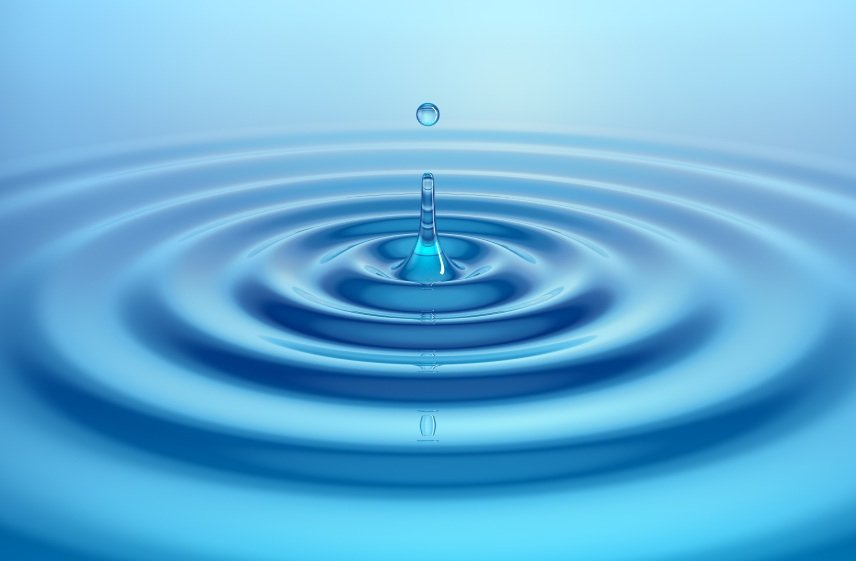
\includegraphics[scale=0.65]{figures/pond_ripple_surface.png}
     \caption[Conceptualizing moderate to worst case error surfaces]{In the case of pond ripples the cost function is defined so that the maxima is the optimal location on the surface. Ripples on a body of water are more challenging to optimize, as the water surfaces are approximately flat on the large scale, yet on the small scale maximas will be temporary preoccupy the GAs learning, but outside of those peaks, there is little large scale information to utilize. }
      
      \label{fig:test1}
\end{center}

\end{figure}


\begin{figure}
      \centering
      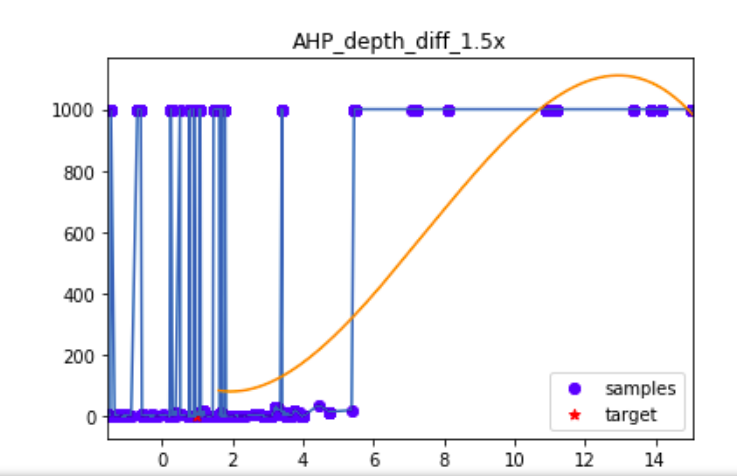
\includegraphics[scale=0.85]{figures/parameter_b_hopeless_surface2.png}
      \caption[Cross section of difficult or hopeless error surface]{Parameter b was slowly varied in the Izhikevich model while all other parameters where held constant, the AHP depth differences at $1.5 \times rheobase$, was computed for each different model parameterisation of \emph{a}, this resulted in a highly  discontinuous error surface, densely populated by local minima. A polynomial regression algorithm (orange trace) shows that if the error function is smoothed it looks convex, but it is very doubtfull that the GA would experience the error as anything but random}
      \label{fig:discontinuous_constraint}
\end{figure}


% Note Help wanted making a professional version, of this known to be unattractive draft/concept figure.
\begin{figure}
\centering
      \label{fig:test1}
      \centering
      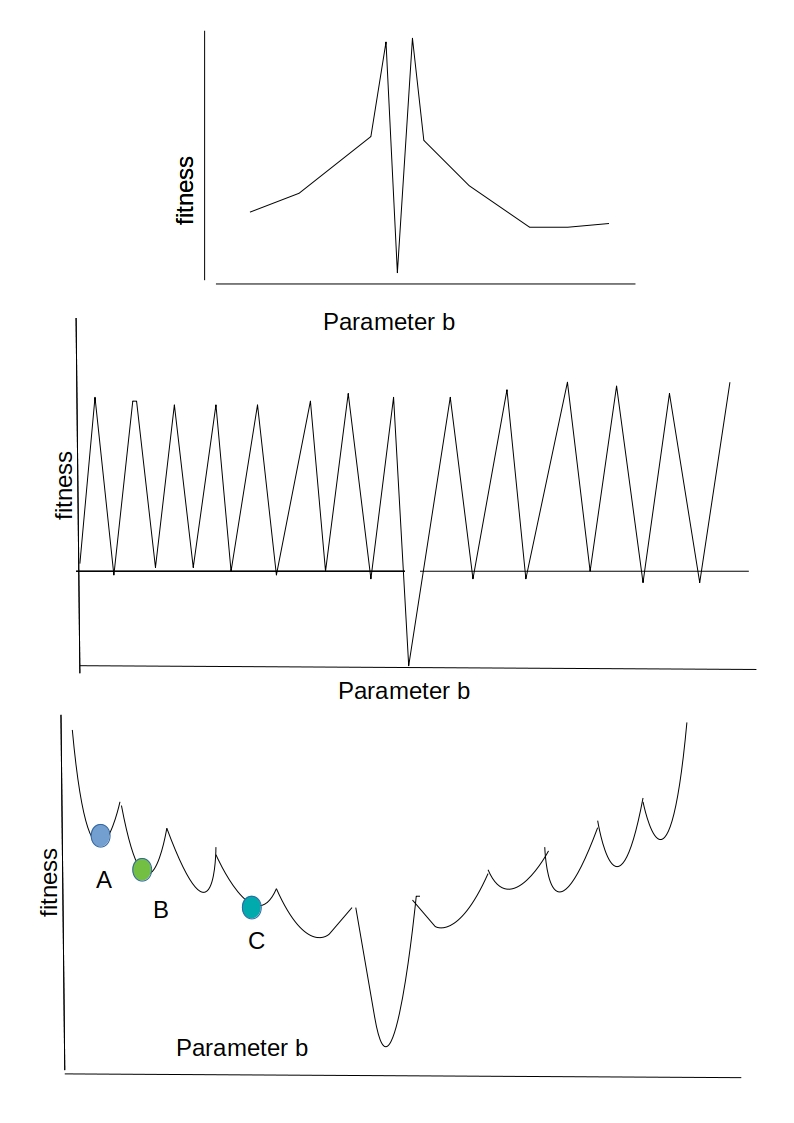
\includegraphics[scale=0.85]{figures/spectrum_worst_error_surfaces2.jpg}
      \caption[Hypothetical Error Functions, Worse than Rastrigrins function]{Rastrigrins function describes a challenging error surface, but one with learnable global features that a genetic algorithm can exploit. Consider the bottom inset figure, which is a cross section of a Rastrigin like function. Along the course of evolution, there is plenty of opportunity for genes like A and B to recombine, often producing fitter children like C. It's important to note that there are much worse error surfaces, and these may show up in practice consider for example the middle inset figure, where cross-over has nothing useful to contribute.
      The situation in the topmost inset is worse again still. In this context learning is a disadvantage, if the optimizer "learns", then it actually slows obtaining an optimal solution, which it can only with a very lucky/just right large random mutation. It is likely that a GA on this surface will be slower than grid search. The second type of error surface actually a 1D (and upside down) cross section of the 2D pond diagram, only actively misleads locally, globally it simply contains no helpful global information. Learning will not be of any assistance in obtaining the optima, but also learning won't be a disadvantage either, the Genetic Algorithm, will simply behave as a random sample testing algorithm, the GA will find the optimum in time, but possibly not as quickly or reliably as exhaustive search would. The second figure is a cross section of the pond ripple argument}
      \label{fig:test2}
\end{figure}

\begin{figure}
\centering
      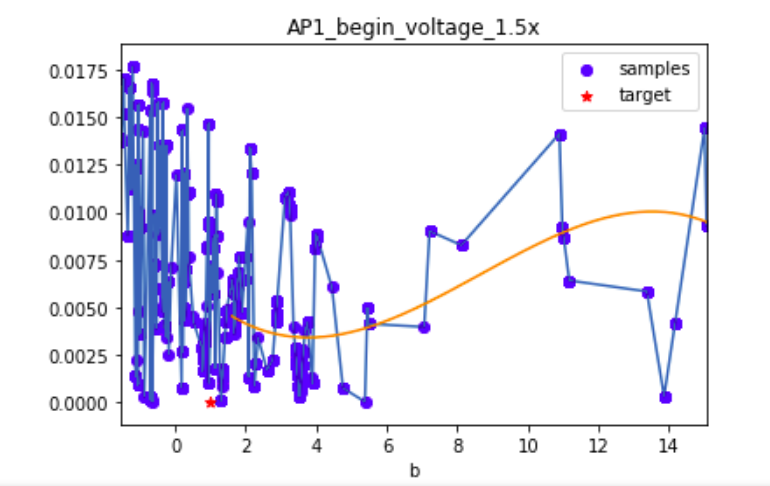
\includegraphics[scale=0.85]{figures/parameter_b_hopeless_surface.png}
      \caption[Cross section of an unhelpful objective function]{Parameter b was slowly varied in the Izhikevich model while all other parameters where held constant, the AP1 begin voltage (threshold), was computed for each different model parameterisation of \emph{a}, this resulted in a highly rippled error surface, densely populated by local minima, and with only a very shallow global convex shape. A polynomial regression algorithm (orange trace), is a very bad fit of the error function. This implies that the function is not very smooth, and seemingly random. The optima value depicted as a red star, is buried in random irregularities in error surface.
    }
      \label{fig:probably_smooth_constraint}
\end{figure}

\begin{figure}      
\centering
      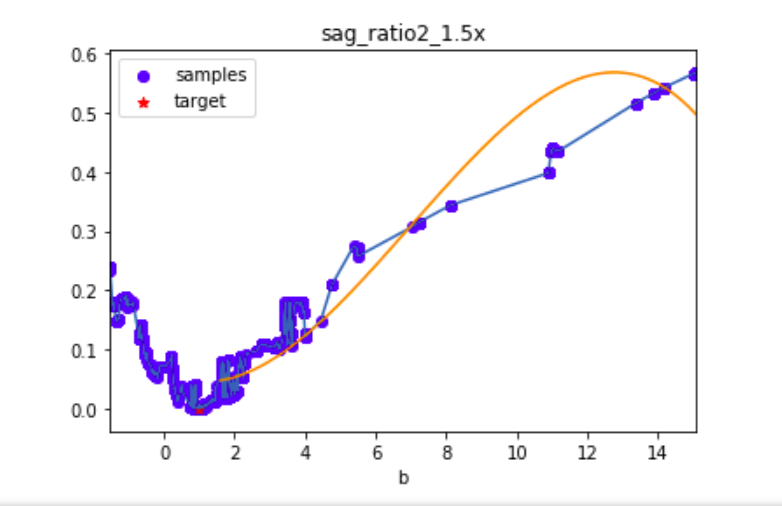
\includegraphics[scale=0.85]{figures/parameter_b_friendly_surface.png}
      \caption[Cross section of an informative and learnable objective function]{
      sag-ratio at 1.5 $\times$ rheobase error is plotted (y-axis) as I sweep across values of b $(x-axis)$. A polynomial regression algorithm (orange trace), is actually a semi reasonable fit of the error function. The quality of it fit entails smoothness.
    
    This is a cross section of a useable and tractable error surface, it has learnable global and local information, as long as not all error surfaces in the multi-objective collection of constraints, this surface is likely to be a valuable addition to the optimizer suite}
      \label{fig:test2}
\end{figure}


   When considering 2D relationships between single parameters and single objective functions, ideally each error function might contribute helpful information, which en-masse boosts the total amount of helpful information. For-instance some 2D error mappings, may contain one or more local minima, but in the same region a different error mapping could lack the error well, meaning that at least one out of two error functions contribute incentive to stride across a minima. The mapping that contains wells, might still be useful to guide optimization, as it may also lack minima in regions were the counterpart has them, additionally the alternative mapping may have regions of $~0.0$ gradient where the other mapping contains significant gradient.
   
   % I am not sure if its impossible to make progress.
 %  Through strategy it is possible to optimize satisfactorily without complete prior knowledge of error surfaces, although such a strategy is not recommended. If prior knowledge of an error surface is prohibited, evolutionary algorithms are definitely a more likely to work than gradient descent.
   
   In a multi objective paradigm, an optimizer could achieve satisfactory solutions when $> \frac{1}{2} \times$ total number of objectives are cogent. In a four objective problem, if the $4$th objective is un-informative, but not actively misleading, inclusion of the 4th objective may only slow down the speed of optimizer convergence.
   
   If the $4$ objective is actively misleading, then a genetic algorithm will likely find a satisfactory solution, by compromising with the dominant $3$ objective functions, and also sampling believed to be "bad" surfaces because of mutation and cross over. Speed of convergence should also be expected to be slower than otherwise. With $\frac{2}{4}$ actively misleading error surfaces, optimization is not expected to work, and it may be slower than psuedo random sampling.
   
   % I don't know if this is true:
   % through good luck you could do heaps of optimization, whithout knowing the error surface.
   % It is almost impossible to make progress without some prior knowledge of the error surfaces, as knowledge of the error surface is a prerequisite for constraining optimization. 
   
   Not all surfaces, provide equally useful information. There are spectrum's of surface quality between convex triangular or parabolic depressions acting as the best solution surfaces, flat functions, and misleading functions. 
   
  
\subsection{Parameter Boundaries}
When setting parameter boundaries there is a dilemma: If the upper and lower parameter margins are closer together than necessary, then optimized models may be deprived of the scope they need to reach their best fit. On the other hand if the boundaries are too far apart, then the governing equations of the model may yield unstable solutions, which may impair the tractibility of the error surface as I will describe below.

Error surface tractability can be compromised in two ways.
Type \textbf{1} solutions to governing equations may contain "not a number" (NaN) or infinity value. The optimizer conventionally interprets more positive numbers as worse. Inside the optimization framework infinity or NaN values are converted to a nominal value of $100.0$, the worst conceivable model score. If more than one gene scores at $100$, then there will be regions of flat error surface. %Although genetic algorithms are not pre-determined to take the steepest path down an error slope, 
%All optimization algorithms are sensitive to the informativeness of error surface, therefore a flat error surface is unhelpful in both gradient descent and genetic algorithms, 

\begin{figure}
    \centering
    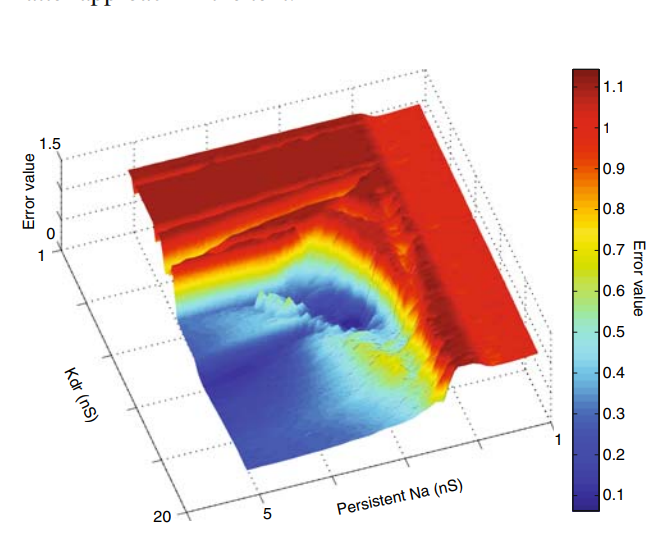
\includegraphics[scale=0.65]{figures/cliff.png}
    \caption[A plot of a cliff ledge framing a 2D error surface]{I include this plot from  literature:
\citep{van2007neurofitter,van2008automated}. It is a plot of summed error across a 2D surface, with swept steps of Na conductance on the x-axis, and $K_{dr}$ conductance on the y-axis. Between Na $[0.75-1]$, you can observe that Na retains a flat value. Presumably the high flat error acts to frame the viable middle region of model parameters, by excluding unstable models.}
    \label{fig:best_at_edge}
\end{figure}
When error surface is flat it is uninformative. Flatness in the viable middle region of optimization, is usually unhelpful, but there is one important place where flatness is helpful. It is warranted for the middle region of error space to be framed by cliffs that demarcate a non-viable perimeter of the error hyper-volume, these are the regions where model parameters are operating slightly beyond their intended scope. There is evidence this approach is used in other optimization work.


\begin{figure}
    \centering
    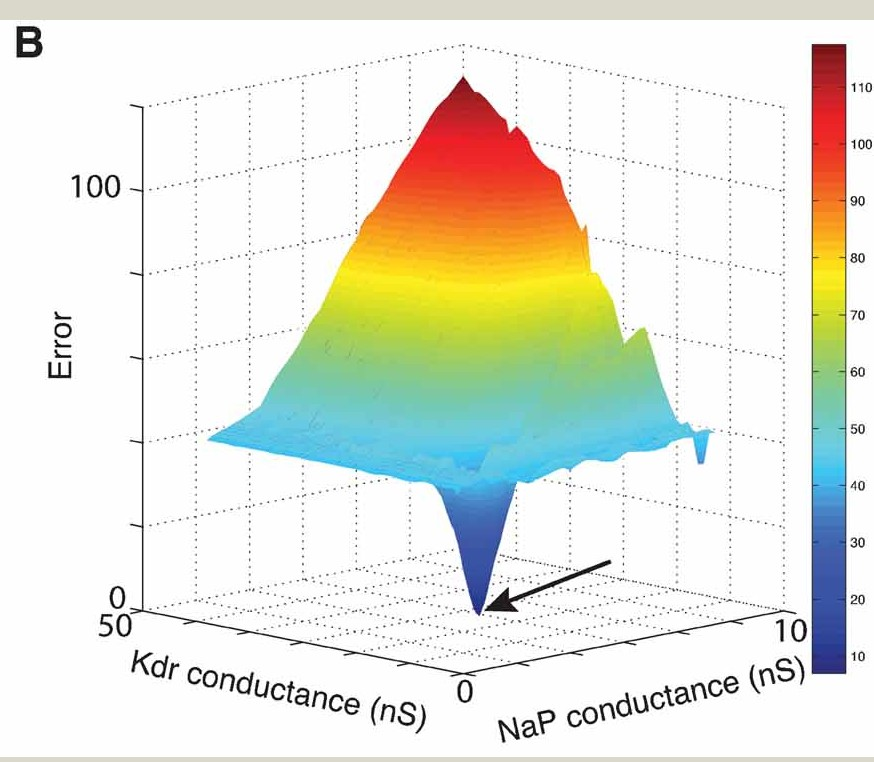
\includegraphics[scale=0.65]{figures/fninf-01-001-g009.jpg}
    \caption[An optimal value that would be missed using only a slim parameter range]{
    Again from the literature I provide a plot of error surface for reduced neuronal models
    \citep{van2008automated}
    \citep{van2007neurofitter}}
    \label{fig:best_at_edge}
\end{figure}

Consider \ref{fig:best_at_edge}, in this figure a global minima is positioned at the intersection two parameter edges in both $Kdr$ and $NaP$. It would be easy to formulate the same optimization problem to have truncated scope about the extremes of $NaP$ and $Kdr$ and as a consequence to miss the uniquely positioned global optima situated on the intersection. The alternative optima that would be reported is the broad spanning region that shares the same second lowest value to the optima. 

%The genetic algorithm
As discussed, model-solution instability can occur when the optimizer samples model parameters that are outside of the models intended scope, or when a model returns a nan value inside its intended scope. It is tempting to think of 

Usually these flat cliffs that neatly encase the error hyper volume like in the figure below \ref{fig:cliff} (and as described above).

% Not helpful for audiance to understand.
%unfortunately however, because each model has a large number of parameters typically $>10$, any particular model instance, only one of these parameters need be evaluating an unstable model when exceeding a margin, the rest of the parameters may be in the middle of their range, and so such a ledge may mostly be experienced as a hyper dimensional "tower", this tower could actually be experienced in the middle of parameter space in 10 out of 11 parameters, while still being on at the edge for only the 11th parameter. The unfortunate consequence of such towers is to lesion in the middle of parameter space inhibits the migration of chromosomes between regions. 

Overall the genetic algorithm is robust, and any middle region discontinuities, are a temporary hindrance that only slow down learning. When considering the GA overall, there are is only a small number of samples that can occur, so the occurrence of middle region lesions in error surface need to reduced  to maximize the informativeness of every precious sample. 

The major strategy for circumvent unnecessary ridges and towers is to pick and chose error functions sparingly and to assess results in a piecemeal basis. Utilizing a "sparing" inclusion policy will have to occur despite the large conflicting incentive to employ as many objective functions as possible.

% Picking the right objective functions will likely involve favoring a-posteri evidence over a-priori arguments about which errors "should" work best. 

%the majority of samples in the middle of the error space.

To supplement figures from the literature, here I include some figures from problems encountered in this work.

Although we are considering single points, and not surfaces, very often if a point is unstable, its neighbours are also unstable, in this way points of instability tend to be a constituents of larger regions of surface that add up to towers, cliffs and ledges such as those in seen here {fig:cliff}.

One or more cliffs or towers situated in the middle of the error surface, poses problems for efficient optimization, where genes learn the general shape of an error surface. %Such cliffs and ledges will mislead the optimizer and they will act exactly like the ripples discussed briefly before in this work.

%Type \textbf{2}: While some towers can be circumvented by choosing slimmer parameter margins, other ledges and ripples of these ledges are implied by the types of model and test combinations. Rather than being avoidable, they are a feature of the complex problem that the optimizer is tasked with solving.

Forinstance, in bursting regimes of the Izhikevich model, where models deliberately produce close to unstable limit cycles. When surpassing the threshold to cause spiking, the slightest increment of current  will illicit not a single spike but a burst of ten.

Rheobase values will be undetermined, because the a  current injection value to that causes only one spike does not exist. The models rheobase value will be assigned to 100, and a tower will punctuate, the error surface possibly in the middle of the Izhikevich parameter hypervolume. The experience of sampling this tower, will visible in evaluation of the  algorithms learning performance. It will likely appear as a one or several unexpected peaks late in the genetic algorithms learning. Also this tower may act to lesion error surface, and to inhibit the movement of chromosomes across the solution space.

This means that even under the most tractible conditions when evaluating the performance of genetic algorithm learning, the rapidity of genetic convergence will vary depending on which constraints are chosen, and the regime that the neuronal model is currently sampling from (the models parameters). There will be regions of genetic learning when models will encode high local pockets of error, or "towers" in the middle of the hyper-volume, and if these towers are significantly wide or densely populated, the genetic algorithms learning will be visibly diminished to a random sampling algorithm. What is more, these discontinuties under some circumstances may act to lesion error surfaces and inhibit migration of models from side to side. Movement over cliffs of course will still ultimately occur due to stochastic pressure in gene mutation.

A possible solution to the dilemma of narrow parameter boundaries is to write an algorithm that slowly samples models by expanding beyond known to stable boundaries, and reports back on model stability. In this manner one can do unsupervised learning of maximum parameter boundaries, however, model equations used here, do exhibit some higher order sensitivity by changing a second intermediate parameter. Very quickly this approach to finding the maximum scope of a parameter may begin to look like exhaustive search.

Another programmatic approach is to use a wide variety of models and tests, and to accept that for some model-test combinations, for some regions of parameter space, genetic algorithms are at worst randomly stumbling upon satisfactory solutions, and at best efficiently learning the optima solutions.
